% Modelo de projeto de dissertação criado para o PPGCC
% da Universidade Federal do Pará a partir da classe abntex2.
% Este documento só deverá ser alterado para incluir ou excluir
% elementos pré e pós textuais. Use o comentário do latex (%) caso
% deseje excluir algum elemento.

%% abtex2-modelo-trabalho-academico.tex, v-1.9.6 laurocesar
%% Copyright 2012-2016 by abnTeX2 group at http://www.abntex.net.br/ 
%%
%% This work may be distributed and/or modified under the
%% conditions of the LaTeX Project Public License, either version 1.3
%% of this license or (at your option) any later version.
%% The latest version of this license is in
%%   http://www.latex-project.org/lppl.txt
%% and version 1.3 or later is part of all distributions of LaTeX
%% version 2005/12/01 or later.
%%
%% This work has the LPPL maintenance status `maintained'.
%% 
%% The Current Maintainer of this work is the abnTeX2 team, led
%% by Lauro César Araujo. Further information are available on 
%% http://www.abntex.net.br/
%%
%% This work consists of the files abntex2-modelo-trabalho-academico.tex,
%% abntex2-modelo-include-comandos and abntex2-modelo-references.bib
%%

% ------------------------------------------------------------------------
% ------------------------------------------------------------------------
% abnTeX2: Modelo de Trabalho Academico (tese de doutorado, dissertacao de
% mestrado e trabalhos monograficos em geral) em conformidade com 
% ABNT NBR 14724:2011: Informacao e documentacao - Trabalhos academicos -
% Apresentacao
% ------------------------------------------------------------------------
% ------------------------------------------------------------------------

\documentclass[
	% -- opções da classe memoir --
	12pt,				% tamanho da fonte
	openright,			% capítulos começam em pág ímpar (insere página vazia caso preciso)
	oneside,			% para impressão em frente e verso. Oposto a oneside
	a4paper,			% tamanho do papel.
	% -- opções da classe abntex2 --
	chapter=TITLE,		% títulos de capítulos convertidos em letras maiúsculas
	%section=TITLE,		% títulos de seções convertidos em letras maiúsculas
	%subsection=TITLE,	% títulos de subseções convertidos em letras maiúsculas
	%subsubsection=TITLE,% títulos de subsubseções convertidos em letras maiúsculas
	% -- opções do pacote babel --
	english,			% idioma adicional para hifenização
	french,				% idioma adicional para hifenização
	spanish,			% idioma adicional para hifenização
	brazil				% o último idioma é o principal do documento
	]{abntex2}

% ---
% Pacotes básicos 
% ---
\usepackage{lmodern}			% Usa a fonte Latin Modern
\usepackage{mathptmx}			% Usa a fonte Times New Roman
\usepackage[T1]{fontenc}		% Selecao de codigos de fonte.
\usepackage[utf8]{inputenc}		% Codificacao do documento (conversão automática dos acentos)
\usepackage{lastpage}			% Usado pela Ficha catalográfica
\usepackage{indentfirst}		% Indenta o primeiro parágrafo de cada seção.
\usepackage{color}				% Controle das cores
\usepackage{graphicx}			% Inclusão de gráficos
\usepackage{subcaption}				% Inclusão de gráficos lado a lado
\usepackage{microtype} 			% para melhorias de justificação
\usepackage{tabularx,ragged2e}	% Para inserir tabelas
\usepackage{multirow}			% Para mesclar células
\usepackage[dvipsnames,table,xcdraw]{xcolor}		% Permite adicionar cores nas linhas de tabelas
\usepackage{fancyvrb}			% Permite adicionar arquivos de texto
\usepackage[portuguese, ruled, linesnumbered]{algorithm2e} % Uso de algoritmos
\usepackage{amsfonts}			% Permite usar notação de conjuntos
\usepackage{amsmath}			% Permite citar equações
\usepackage{amsthm}				% Permite criar teoremas e experimentos
\usepackage[font={bf, small}, labelsep=endash, labelfont=bf]{caption}	% Faz legenda de figuras ficarem em negrito
\usepackage{cancel}				% Permite fazer expressão tendendo a zero
\usepackage{epstopdf}			% Converte eps para pdf
\usepackage[final]{pdfpages}

\newcolumntype{L}{>{\RaggedRight\arraybackslash}X}
% ---

% ---
% Pacotes de citações
% ---
%\usepackage[brazilian,hyperpageref]{backref}	 % Paginas com as citações na bibl
\usepackage[alf, abnt-emphasize=bf]{abntex2cite}	% Citações padrão ABNT

% ---
% Customizações para o layout da UFPA
% ---
\usepackage{modelo-ufpa/ufpa}

% Muda o título das listas
\addto\captionsbrazil{%
  \renewcommand{\listfigurename}%
    {Lista de Ilustrações}%
	\renewcommand{\listtablename}%
    {Lista de Tabelas}%
}

% Permite utilizar figuras sem precisar colocar o caminho absoluto
\graphicspath{{imagens/}}

% --- 
% CONFIGURAÇÕES DE PACOTES
% --- 

% ---
% Configurações do pacote backref
% Usado sem a opção hyperpageref de backref
%\renewcommand{\backrefpagesname}{Citado na(s) página(s):~}
% Texto padrão antes do número das páginas
%\renewcommand{\backref}{}
% Define os textos da citação
%\renewcommand*{\backrefalt}[4]{
%	\ifcase #1 %
%		Nenhuma citação no texto.%
%	\or
%		Citado na página #2.%
%	\else
%		Citado #1 vezes nas páginas #2.%
%	\fi}%
% ---

% ---
% Informações de dados para CAPA e FOLHA DE ROSTO
% ---
\universidade{UNIVERSIDADE FEDERAL DO PARÁ}
\instituto{INSTITUTO DE CIÊNCIAS EXATAS E NATURAIS}
\programa{PROGRAMA DE PÓS-GRADUAÇÃO EM CIÊNCIA DA COMPUTAÇÃO}
\titulo{\textcolor{red}{<Título do Projeto de Dissertação>}}
\autor{\textcolor{red}{<NOME DO ALUNO>}}
\local{Belém}
\data{\textcolor{red}{<Ano>}}
\orientador{\textcolor{red}{<Nome do Professor>}}
\tipotrabalho{Projeto de Dissertação}
% O preambulo deve conter o tipo do trabalho, o objetivo, 
% o nome da instituição e a área de concentração 
\preambulo{Projeto de Dissertação de Mestrado apresentado ao Programa de Pós-Graduação em Ciência da Computação. Instituto de Ciências Exatas e Naturais. Universidade Federal do Pará.}
\areadeconcentracao{\textcolor{red}{<Nome da Área>}}
\newcommand{\imprimirfaculdadedoorientador}{Faculdade de Biotecnologia - UFPA}
\newcommand{\imprimirprimeiromembrodabanca}{Prof. Dr. Nelson Cruz Sampaio Neto}
\newcommand{\imprimirfaculdadedoprimeiromembrodabanca}{Faculdade de Computação - UFPA}
\newcommand{\imprimirsegundomembrodabanca}{Prof. Dra. Adriana Ribeiro Carneiro}
\newcommand{\imprimirfaculdadedosegundomembrodabanca}{Faculdade de Biotecnologia - UFPA}
\newcommand{\imprimirpalavraschave}{%
1. Bioinformática.
2. Curadoria de genomas.
3. Fechamento de gaps.
}
% ---


% ---
% Configurações de aparência do PDF final

% alterando o aspecto da cor azul
\definecolor{blue}{RGB}{41,5,195}

% informações do PDF
\makeatletter
\hypersetup{
     	%pagebackref=true,
		pdftitle={\imprimirtitulo}, 
		pdfauthor={\imprimirautor},
    	pdfsubject={\imprimirpreambulo},
	    pdfcreator={LaTeX with abnTeX2},
		pdfkeywords={\imprimirpalavraschave}, 
		colorlinks=true,       		% false: boxed links; true: colored links
    	linkcolor=black,          	% color of internal links
    	citecolor=black,        		% color of links to bibliography
    	filecolor=magenta,      		% color of file links
		urlcolor=blue,
		bookmarksdepth=4,
        breaklinks=true
}
\makeatother
% --- 

% --- 
% Espaçamentos entre linhas e parágrafos 
% --- 

% O tamanho do parágrafo é dado por:
\setlength{\parindent}{1.3cm}

% Controle do espaçamento entre um parágrafo e outro:
\setlength{\parskip}{0.2cm}  % tente também \onelineskip

% ---
% compila o indice
% ---
\makeindex
% ---

% ----
% Início do documento
% ----
\begin{document}

% Seleciona o idioma do documento (conforme pacotes do babel)
%\selectlanguage{english}
\selectlanguage{brazil}

% Retira espaço extra obsoleto entre as frases.
\frenchspacing 

% ----------------------------------------------------------
% ELEMENTOS PRÉ-TEXTUAIS
% ----------------------------------------------------------
% \pretextual

% ---
% Capa
% ---
\imprimircapa
% ---

% ---
% Folha de rosto
% ---
\imprimirfolhaderosto
% ---

\newpage

% ---
% inserir lista de ilustrações
% ---
\pdfbookmark[0]{\listfigurename}{lof}
\listoffigures*
\cleardoublepage
% ---

% ---
% inserir lista de tabelas
% ---
\pdfbookmark[0]{\listtablename}{lot}
\listoftables*
\cleardoublepage
% ---

% ---
% inserir lista de abreviaturas e siglas
% ---
\begin{siglas}
	\item[\textcolor{red}{<Sigla>}] \textcolor{red}{<Definição>}
\end{siglas}
% ---

% ---
% inserir o sumario
% ---
\pdfbookmark[0]{\contentsname}{toc}
\tableofcontents*
\cleardoublepage
% ---



% ----------------------------------------------------------
% ELEMENTOS TEXTUAIS
% ----------------------------------------------------------
\textual

% ----------------------------------------------------------
% Introdução
% ----------------------------------------------------------
\chapter{Introdução}
\label{cap:introducao}

\textcolor{red}{<Descrever sucintamente o contexto do Projeto de Dissertação, bem como apresentar os principais assuntos a serem discutidos ao longo do documento: objetivos e metas do projeto.>}

\section{Exemplos de uso de figuras, gráficos, referências e citações}

A estrutura da molécula de DNA tem formato helicoidal \cite{watson1953molecular}. Um exemplo é ilustrado na \autoref{fig:dna}.

\begin{figure}[!htb]
	\caption{Estrutura da molécula de DNA}
	\label{fig:dna}
	\centering
	
\includegraphics[width=.3\textwidth]{estrutura_dna.eps} \\
	\begin{small}\textbf{Fonte: \citeonline{watson1953molecular}}\end{small}
\end{figure}

\subsection{Definindo subseções}

\begin{grafico}[!htb]
	\caption{Projetos de sequenciamento de genomas cadastrados no banco de dados GOLD}
	\label{grafico:gold}
	\centering
	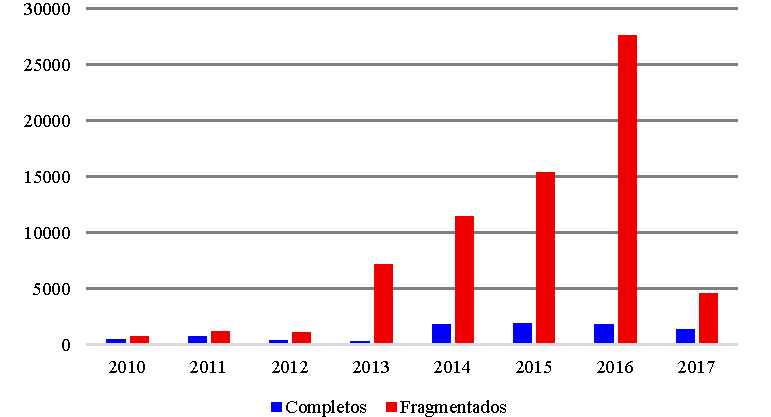
\includegraphics[width=.8\textwidth]{gold.pdf} \\
	\begin{small}\textbf{Fonte: \citeonline{mukherjee2016}}\end{small}
\end{grafico}

\chapter{Contextualização e Terminologias do Trabalho}
\label{cap:contextualizacao}

\textcolor{red}{<Apresentar um detalhado Estado da Arte sobre o assunto do Projeto de Dissertação.> }

\chapter{Trabalhos Relacionados}
\label{cap:trabalhosrelacionados}

\textcolor{red}{<Apresentar os Trabalhos Relacionados no contexto do desenvolvimento da pesquisa, detalhando os Pontos Fortes, Fracos e Melhorias.>}

\chapter{Motivação}
\label{cap:motivacao}

\textcolor{red}{<Descrever de maneira detalhada a principal motivação para a realização do trabalho de pesquisa, caracterizando a problemática do trabalho.>}

\chapter{Justificativa e Contribuição à Área}
\label{cap:justificativa}

\textcolor{red}{<Apresentar claramente a justificativa para o desenvolvimento do projeto, alinhado à problemática descrita na seção anterior, bem como apresentar as principais contribuições para a área de pesquisa quando do desenvolvimento do trabalho.>}

\chapter{Objetivos}
\label{cap:objetivos}

\textcolor{red}{<Deve-se apresentar os Objetivos Geral e Específicos para o desenvolvimento do trabalho.>}

\section{Objetivo Geral}

\textcolor{red}{<Descrever o Objetivo Geral do trabalho, alinhado à justificativa apresentada na seção anterior e aderente à contribuição definida.>}

\section{Objetivos Específicos}

\textcolor{red}{<Listar os principais objetivos específicos, alinhados ao Objetivo Geral. Não confundir objetivos específicos com as metas do trabalho.>}

\chapter{Forma de Validação}
\label{cap:validacao}

\textcolor{red}{<Descrever detalhadamente a forma como a proposta do projeto será validada. Vale analisar e instanciar alguns métodos, propostos nas literaturas especializadas, usados para formalizar os resultados a serem obtidos com o desenvolvimento do projeto.>}

\chapter{Metodologia de Pesquisa}
\label{cap:metodologia}

\textcolor{red}{<Descrever a metodologia científica usada para a realização da pesquisa, detalhando as etapas a serem executadas para o desenvolvimento do projeto.>}

\chapter{Cronograma}
\label{cap:cronograma}

\textcolor{red}{<Relacionar as principais atividades a serem realizadas no desenvolvimento do projeto e definir prazos para as suas conclusões. Importantes estas atividades estarem alinhadas com as etapas descritas na metodologia definida na seção anterior.>}

\begin{table}[!htb]
	\caption{Cronograma de execução do projeto}
	\label{tab:cronograma}
	\centering
	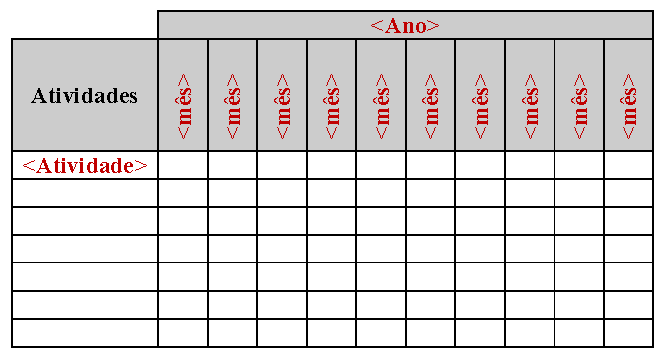
\includegraphics[width=1\textwidth]{cronograma.pdf} \\
	\begin{small}\textbf{Fonte: O Autor (2017)}\end{small}
\end{table}


% ----------------------------------------------------------
% ELEMENTOS PÓS-TEXTUAIS
% ----------------------------------------------------------
\postextual
% ----------------------------------------------------------

% ----------------------------------------------------------
% Referências bibliográficas
% ----------------------------------------------------------
\bibliography{bibliografia}
% ---

\end{document}
